%%%%%%%%%%%%%%%%%%%%%%%%%%%%%%%%%%%%%%%%%
% Journal Article
% LaTeX Template
% Version 1.4 (15/5/16)
%
% This template has been downloaded from:
% http://www.LaTeXTemplates.com
%
% Original author:
% Frits Wenneker (http://www.howtotex.com) with extensive modifications by
% Vel (vel@LaTeXTemplates.com)
%
% License:
% CC BY-NC-SA 3.0 (http://creativecommons.org/licenses/by-nc-sa/3.0/)
%
%%%%%%%%%%%%%%%%%%%%%%%%%%%%%%%%%%%%%%%%%

%----------------------------------------------------------------------------------------
%	PACKAGES AND OTHER DOCUMENT CONFIGURATIONS
%----------------------------------------------------------------------------------------

\documentclass[twoside,twocolumn]{article}
  
  \usepackage{blindtext} % Package to generate dummy text throughout this template 
  \usepackage[sc]{mathpazo} % Use the Palatino font
  \usepackage[T1]{fontenc} % Use 8-bit encoding that has 256 glyphs
  \linespread{1.05} % Line spacing - Palatino needs more space between lines
  \usepackage{microtype} % Slightly tweak font spacing for aesthetics
  
  \usepackage[english]{babel} % Language hyphenation and typographical rules
  \usepackage[hmarginratio=1:1,top=32mm,columnsep=20pt]{geometry} % Document margins
  \usepackage[hang, small,labelfont=bf,up,textfont=it,up]{caption} % Custom captions under/above floats in tables or figures
  \usepackage{booktabs} % Horizontal rules in tables
  
  \usepackage{lettrine} % The lettrine is the first enlarged letter at the beginning of the text
  
  \usepackage{enumitem} % Customized lists
  \setlist[itemize]{noitemsep} % Make itemize lists more compact
  
  \usepackage{abstract} % Allows abstract customization
  \renewcommand{\abstractnamefont}{\normalfont\bfseries} % Set the "Abstract" text to bold
  \renewcommand{\abstracttextfont}{\normalfont\small\itshape} % Set the abstract itself to small italic text
  
  \usepackage{titlesec} % Allows customization of titles
  \renewcommand\thesection{\Roman{section}} % Roman numerals for the sections
  \renewcommand\thesubsection{\roman{subsection}} % roman numerals for subsections
  \titleformat{\section}[block]{\large\scshape\centering}{\thesection.}{1em}{} % Change the look of the section titles
  \titleformat{\subsection}[block]{\large}{\thesubsection.}{1em}{} % Change the look of the section titles
  
  \usepackage{tikz}
  \usetikzlibrary{arrows.meta,automata,positioning}
  
  \usepackage{fancyhdr} % Headers and footers
  \pagestyle{fancy} % All pages have headers and footers
  % \fancyhead{} % Blank out the default header
  \fancyfoot{} % Blank out the default footer
  % \fancyhead[C]{Running title $\bullet$ May 2016 $\bullet$ Vol. XXI, No. 1} % Custom header text
  \fancyfoot[RO,LE]{\thepage} % Custom footer text
  
  \usepackage{titling} % Customizing the title section
  
  \usepackage{hyperref} % For hyperlinks in the PDF
  
  \usepackage{xcolor}
  \usepackage{tabu}
  \usepackage{hyperref}  
  \usepackage{colortbl}
  
  \usepackage{amsmath}
  \usepackage{algorithm}
  \usepackage[noend]{algpseudocode}
  
  \usepackage{wrapfig}
  
  \usepackage{selinput}
  \SelectInputMappings{%
    aacute={á},
    oacute={ó},
    iacute={í},
    ntilde={ñ},
    Euro={€}
  }
  
  \newcommand\nth{\textsuperscript{th}\xspace} %\th is taken already
  
  %----------------------------------------------------------------------------------------
  %	TITLE SECTION
  %----------------------------------------------------------------------------------------
  
  
  \setlength{\droptitle}{-4\baselineskip} % Move the title up
  
  \pretitle{\begin{center}\Huge\bfseries} % Article title formatting
  \posttitle{\end{center}} % Article title closing formatting
  \title{Solving the Traveling Salesman Problem: a multithreaded approach with evolutionary genetic algorithms} % Article title
  \author{%
  \textsc{Ibsan Acis Castillo Vitar} \\[1ex] % Your name
  \normalsize School of Sciences and Engineering, Tecnológico de Monterrey, Puebla Campus \\ % Your institution
  \normalsize \href{mailto:A01014779@itesm.mx}{A01014779@itesm.mx} % Your email address
  \and % Uncomment if 2 authors are required, duplicate these 4 lines if more
  \textsc{Luis Fernando Dávalos Domínguez} \\[1ex] % Second author's name
  \normalsize School of Sciences and Engineering, Tecnológico de Monterrey, Puebla Campus \\ % Your institution
  \normalsize \href{mailto:A01128697@itesm.mx}{A01128697@itesm.mx} % Second author's email address
  \and % Uncomment if 2 authors are required, duplicate these 4 lines if more
  \textsc{Salvador Orozco Villalever} \\[1ex] % Second author's name
  \normalsize School of Sciences and Engineering, Tecnológico de Monterrey, Puebla Campus \\ % Your institution
  \normalsize \href{mailto:A07104218@itesm.mx}{A07104218@itesm.mx} % Second author's email address
  }
  \date{November 13\nth 2017} % Leave empty to omit a date
  \renewcommand{\maketitlehookd}{%
  \begin{abstract}
  \noindent The Traveling Salesman Problem is a one of the most common NP-Complete problems. As one of the most complicated problems in the history of Computer Science, there currently are no algorithms that can solve it in polynomial time. The problem's description is simple: given $N$ cities that a salesman has to visit, find the order in which he must visit them to minimize the total distance traveled if he has to visit all cities once and come back to the first city after visiting the last one. For each number of cities $N$, the number of permutations of cities is $N!$, which makes the problem's size grow very fast. We approach the problem via genetic algorithms. 
  \end{abstract}
  }
  
  %----------------------------------------------------------------------------------------
  
  \begin{document}
  
  % Print the title
  \maketitle
  
  %----------------------------------------------------------------------------------------
  %	ARTICLE CONTENTS
  %----------------------------------------------------------------------------------------
  
  \section{Introduction}
  
  \lettrine[nindent=0em,lines=3]{T}he goal of this project is to obtain the optimal solution for the Traveling Salesman Problem, a problem that consists of a salesman and a set of cities which have to be visited. The salesman has to visit each city once and return to the same city after the last one has been visited.\linebreak
  
  Consider the following image. The problem lies in finding the shortest path visiting all vertices once. For example the path $1$:${A,C;D,B,A}$ and $2$:${A,B,C,D,A}$ visit all the vertices once, but path $1$ has a length of $108$ while path $2$ has a length of $97$.\linebreak
  
  \begin{tikzpicture}[
        > = stealth, % arrow head style
        shorten > = 1pt, % don't touch arrow head to node
        auto,
        node distance = 1.5 cm, % distance between nodes
        semithick % line style
      ]
  
      \tikzset{every state}=[
        draw = black,
        thick,
        fill = white,
        minimum size = 1mm
      ]
  
      \node[state] (C) {$C$};
      \node[state] (D) [right=of C] {$D$};
      \node[state] (A) [above=of C]{$A$};
      \node[state] (B) [above=of D] {$B$};
    
      \path[-] (A) edge  node[] {20} (B);
      \path[-] (A) edge  node[] {42} (C);
      \path[-] (A) edge  node[pos=0.20, above] {35} (D);
      
      \path[-] (B) edge  node[pos=0.20, below] {30} (C);
      \path[-] (B) edge  node[] {34} (D);
      
      \path[-] (C) edge  node[] {12} (D);
  \end{tikzpicture}
      
  The number of cities in this problem is $4$, and there are $4! = 24$ possible routes, which makes the problem very complex as the number of cities grow.\linebreak
  
  We approach this problem with evolutionary genetic algorithms. We receive the number of cities and their geographic coordinates. We calculate the distance between cities using the Haversine distance formula.\linebreak
  
  %------------------------------------------------
  
  \section{Mathematical Formulation}
  
  For a given $n \times n$ distance matrix $C = (c_{ij})$, find a cyclic permutation $\pi$ of the set $\{1, 2, ..., n\}$ that minimizes the function
  
  \begin{equation}
  c(\pi) = \sum_{i=1}^{n} C_{i\pi(i)}
  \end{equation}
  
  where $c(\pi)$ is the length of the permutation $\pi$, computed through a distance metric. In our case, the metric is the Haversine formula to calculate the distance between two fixed points on Earth given the latitude and longitude of each point.
  %------------------------------------------------
  
  \section{Related Work}
  
  The Traveling Salesman Problem was first considered mathematically in the 1930s by Merrill Floyd. In the 1950s and 1960s, the problem became increasingly popular in scientific circles in Europe and the USA. Notable contributions were made by George Dantzig, Delbert Ray Fulkerson and Selmer M. Johnson; they expressed the problem as an integer linear programming problem and developed the cutting plane method.\linebreak
  
  In the following decades, the problem was studied by many researchers from mathematics, computer science, chemistry, physics and other sciences.\linebreak
  
  A chemist, V. Černý, created a thermodynamical approach to the Traveling Salesman Problem. He created a Monte Carlo algorithm to find approximate solutions of the TSP. The algorithm generates random permutations, with probability depending on the length of the corresponding route. Reasoning by analogy with statistical thermodynamics, it uses the probability given by the Boltzmann-Gibbs distribution. Using that method they could get very close to the optimal solution.\linebreak
  
  %------------------------------------------------
  
  \section{Methods}
  
  \subsection{Input}
  The input to the program is a text file containing a line with an integer $N$, the number of cities the traveling salesman has to visit. The next $N$ lines contain each two floating-point numbers corresponding to the latitude and longitude of the $i$-th city for $i = 1,2,...,N$.
  
  \subsection{Output}
  The output of the program is the best generated chromosome in terms of the distance required to visit all cities and come back to the first one.
  
  \subsection{Algorithm} 
  The algorithm used to solve this problem is as follows:
  
  \subsubsection{Genetic Algorithm with Ordered Crossover}
  
  \begin{algorithm}
          \caption{Genetic Algorithm with ordered crossover}\label{ga}
          {\fontsize{6}{6}\selectfont \begin{algorithmic}[1]
              \Procedure{Genetic Algorithm with ordered crossover}{}
              \State Set $C$, the total amount of chromosomes per generation
              \State Create $C$ chromosomes each with a random permutation
              \State Set $G$, the total amount of chromosome generations 
              \For{$i\gets 0, G - 1$}  
                \State Sort the array with the $C$ chromosomes at generation $i$
                  \State Let the first $\frac{C}{4}$ \textit{elite} chromosomes live to the next generation
                  \State Create $\frac{3C}{4}$ child chromosomes from the $\frac{C}{4}$ \textit{elite} chromosomes
            
              \EndFor
              \State Sort the array of chromosomes one last time
              \State\textbf{return} the first chromosome in the array
              \EndProcedure
          \end{algorithmic}}
      \end{algorithm}
  
  \subsubsection{Pairing Schema}
  
  Use the following pairing schema to generate child chromosomes:
  
  \begin{enumerate}
  \item The $i$-th chromosome with the $(i + 1)$-th chromosome $\left(1\leq i \leq \frac{C}{4}\right)$
  \item The $i$-th chromosome with the $(i + 2)$-th chromosome $\left(1\leq i \leq \frac{C}{4}\right)$
  \item The $i$-th chromosome with the $(i + 3)$-th chromosome $\left(1\leq i \leq \frac{C}{4}\right)$
  \end{enumerate} 
  
  \textit{Note: all indices are taken modulo $\frac{C}{4}$.}
  
  \subsubsection{Ordered Crossover}
  
  Perform the ordered crossover in the following fashion:
  
  \begin{algorithm}
          \caption{Ordered crossover}\label{oc}
          {\fontsize{6}{6}\selectfont \begin{algorithmic}[1]
              \Procedure{Ordered crossover}{permutation1, permutation2}
              \State Select a random range $\big[i, j\big]$ of the first parent's permutation of cities
              \State Place those $(j - i + 1)$ cities in the same range of the child permutation
              \State Get the remaining cities from the other parent’s permutation in the same order in which they appear
              \State \textbf{return} the new permutation
              \EndProcedure
          \end{algorithmic}}
  \end{algorithm}
  
  \subsubsection{Multithreading}
  
  \begin{algorithm}
          \caption{Multithreading}\label{oc}
          {\fontsize{7}{7}\selectfont \begin{algorithmic}[1]
              \Procedure{Multithreading}{}
              \State Set $P$, the number of processors to be used.
              \State Create an array of $P$ threads
              \For{$i\gets 0, P - 1$}  
                \State Start the $i$-th thread
                \State Let the $i$-th thread execute $threadSolution\big(\big)$ 
                \State Let the $i$-th thread call $solve\big(\big)$
                \State Let the $i$-th thread print its winning chromosome
              \EndFor
              \EndProcedure
          \end{algorithmic}}
  \end{algorithm}

\subsection{Time Complexity Analysis}

\begin{table}[H]
\centering
\fontsize{7}{7}\selectfont
\label{my-label}
\begin{tabular}{|l|l|l|l|}
\hline
 \textbf{ID} & \textbf{Operation} & \textbf{Complexity} \\ \hline
 1 & Creating $C$ random chromosomes & $\mathcal{O}(C^2N)$ \\ \hline
 2 & Sorting the array of $C$ chromosomes & $\mathcal{O}(C\log{C})$ \\ \hline
 3 & Creating $\frac{3C}{4}$ child chromosomes $G$ times & $\mathcal{O}(CNG)$ \\ \hline
 4 & Multithreading & $\mathcal{O}(P)$ \\ \hline
\end{tabular}
\caption{Complexity Analysis of the Algorithm}
\end{table}

As we set the amount of chromosome generations $G$ as $10000$ and the amount of chromosomes per generation $C$ as $100$ in all cases, we can see that operation $3$ has the highest time complexity. Thus,  $\mathcal{O}(CNG)$ is the complexity of our algorithm, where $C$, $N$ and $G$ are the amount of chromosomes per generation, the amount of cities in the input and the amount of generations, respectively.
  
  %------------------------------------------------
  
  \section{Results}
  
  
\subsection{Solutions found}

\taburowcolors[2]{white .. black!20}
  \sffamily\footnotesize
  \tabulinesep=6pt
  \begin{table}[H]
  \begin{tabu}{|>{\cellcolor{black!60}\color{white}}r|X[cm]|X[cm]|}
  \hline
  \rowcolor{black!80}\strut  & \multicolumn{2}{c|}{\color{white} Min. Distance (km)}  \\
  \rowcolor{black!80}\strut Input size (cities) & \color{white}1 core & \color{white}4 cores\\
  10 & 46657.151 & 46657.151\\
  \cline{2-3}
  15 & 48277.834 & 48277.834\\ 
  \hline
  20 & 55175.629 & \textcolor{red}{56012.943}\\
  \cline{2-3}
  25 & 70104.307 & \textcolor{red}{70513.449}\\
  \hline
  \end{tabu}
    \caption{Comparison of solutions found across all four sets of input}
  \end{table}
  
  \taburowcolors[2]{white .. black!20}
  \sffamily\footnotesize
  \tabulinesep=6pt
  \begin{table}[H]
  \begin{tabu}{|>{\cellcolor{black!60}\color{white}}r|X[cm]|X[cm]|}
  \hline
  \rowcolor{black!80}\strut  & \multicolumn{2}{c|}{\color{white}CPU Time (s)}  \\
  \rowcolor{black!80}\strut Input size (cities) & \color{white}1 core & \color{white}4 cores\\
  10 & 67 & 11\\
  \cline{2-3}
  15 & 78 & 13\\ 
  \hline
  20 & 90 & 14\\
  \cline{2-3}
  25 & 101 & 13\\
  \hline
  \end{tabu}
    \caption{Performance comparison across four sets of input}
  \end{table}
  
\subsection{Screenshots of the program execution}

\begin{figure}[H]
\centering
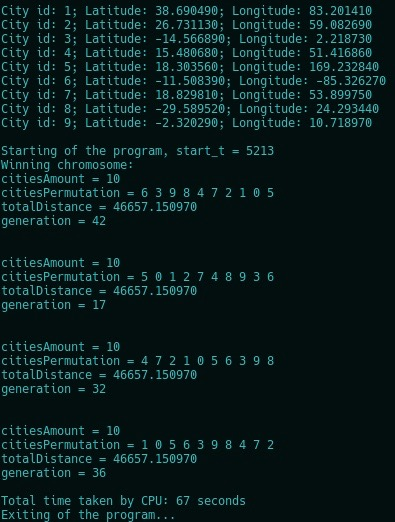
\includegraphics[width=0.45\textwidth]{output1_1_singleThread_10Cities.jpg}
\caption{Output of the single-threaded program with $10$ cities as input}
\end{figure} 

\begin{figure}[H]
\centering
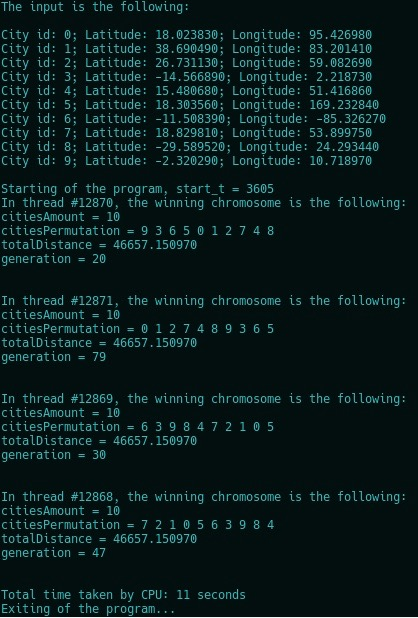
\includegraphics[width=0.45\textwidth]{output1_2_multiThread_10Cities.jpg}
\caption{Output of the multi-threaded program with $4$ cores and $10$ cities as input}
\end{figure} 

\begin{figure}[H]
\centering
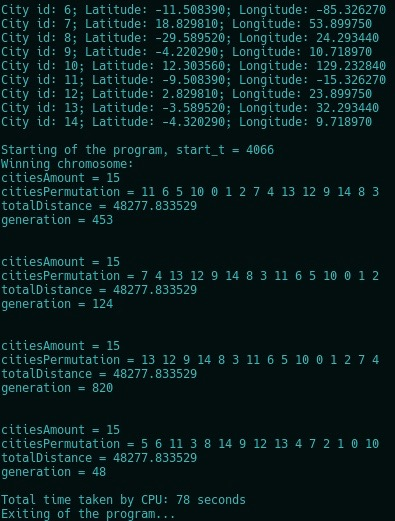
\includegraphics[width=0.45\textwidth]{output2_1_singleThread_15Cities.jpg}
\caption{Output of the single-threaded program with $15$ cities as input}
\end{figure} 

\begin{figure}[H]
\centering
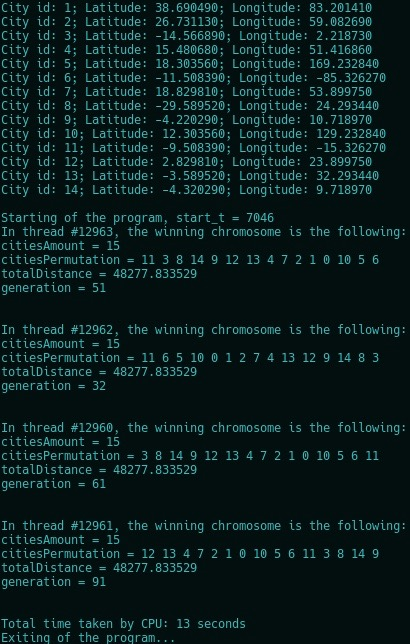
\includegraphics[width=0.45\textwidth]{output2_2_multiThread_15Cities.jpg}
\caption{Output of the multi-threaded program with $4$ cores and $15$ cities as input}
\end{figure}

\begin{figure}[H]
\centering
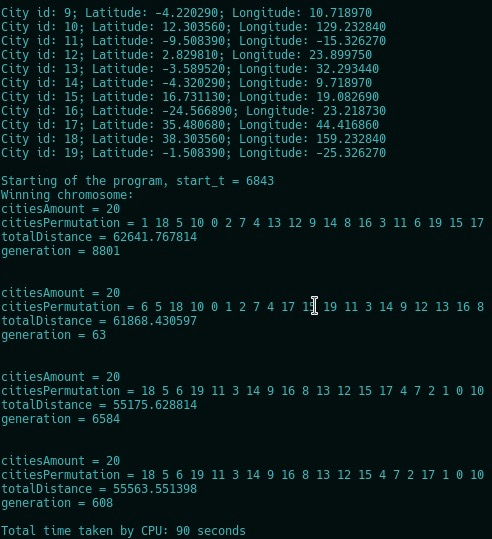
\includegraphics[width=0.45\textwidth]{output3_1_singleThread_20Cities.jpg}
\caption{Output of the single-threaded program with $20$ cities as input}
\end{figure} 

\begin{figure}[H]
\centering
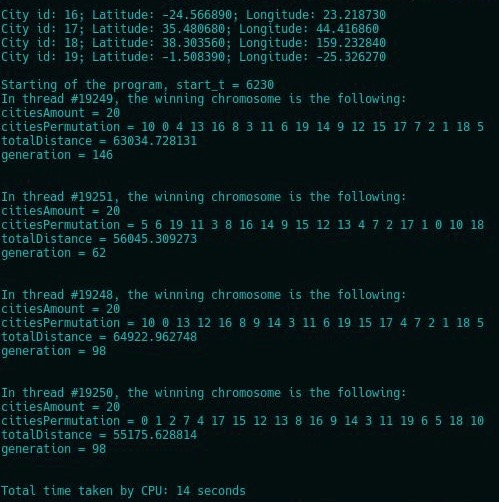
\includegraphics[width=0.45\textwidth]{output3_2_multiThread_20Cities.jpg}
\caption{Output of the multi-threaded program with $4$ cores and $20$ cities as input}
\end{figure} 

\begin{figure}[H]
\centering
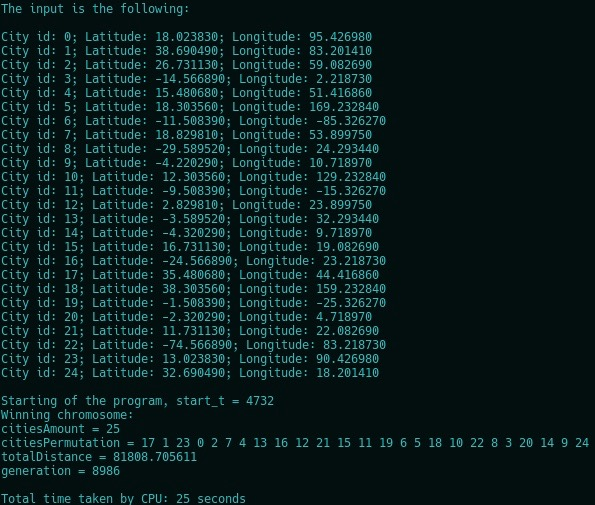
\includegraphics[width=0.50\textwidth]{output4_1_singleThread_25Cities.jpg}
\caption{Output of the single-threaded program with $25$ cities as input}
\end{figure} 

\begin{figure}[H]
\centering
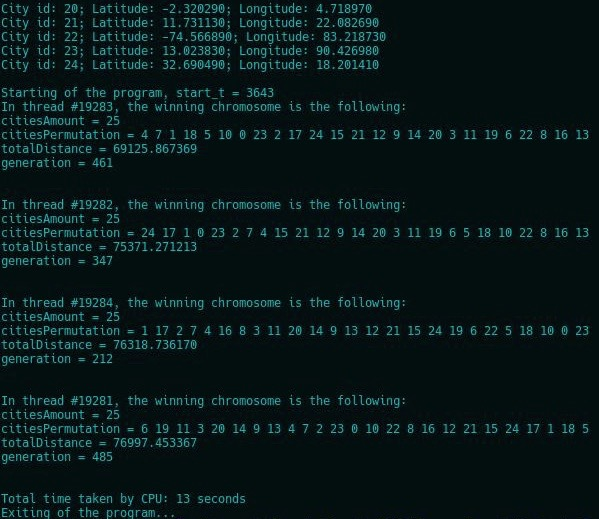
\includegraphics[width=0.50\textwidth]{output4_2_multiThread_25Cities.jpg}
\caption{Output of the multi-threaded program with $4$ cores and $25$ cities as input}
\end{figure} 
  
%------------------------------------------------
  
\section{Discussion}
  
We can see that in all four cases, the multi-threaded approach is around six times faster than the single-threaded one, taking into account that the former version of the program finds four solutions separately, while the latter finds four consecutively. It is also important to notice that both versions of the program get the same answers for the first two input cases, whereas the single-threaded approach beats the multi-threaded one for the last two cases by margins of 0.809$\%$ and $0.584\%$, respectively. We suspect that these last differences in the results have to do with the random nature of the algorithm. Besides, with the single-thread version we have four cores working on the same problem, whereas with the multi-thread version each thread is working on its own. Further analysis and testing should clarify if our idea is true. In the end, it's a tradeoff between speed and accuracy.\linebreak

At first, we hadn't considered rotations of the same cycle as possibilities to reach the same output. However, after a few tests we discovered this, although we also discovered cases in which a two different permutations (none of which is a cycle of the other) reached the same total distance, thus being both valid solutions.
%-------------------------------------------------
  
\section{Conclusion}
  
The Traveling Salesman Problem is a very interesting problem not only because it concerns daily tasks in the lives of lots of people, but also because of its difficult nature, yet simple description. Although we were a bit afraid to tackle such a problem, we think that, in the end, we developed a solution which could be good enough for general purposes. Nevertheless, if we were to use the program's results for scientific or more serious purposes, we would have to work on the logic of the child generation and the ordered crossover, while also thinking deeper in the amount of generations and the amount of chromosomes per generation.
  
  %----------------------------------------------------------------------------------------
  %	REFERENCE LIST
  %----------------------------------------------------------------------------------------
  
  \begin{thebibliography}{99} % Bibliography - this is intentionally simple in this template
  
  % \bibitem[Figueredo and Wolf, 2009]{Figueredo:2009dg}
  % Figueredo, A.~J. and Wolf, P. S.~A. (2009).
  % \newblock Assortative pairing and life history strategy - a cross-cultural
  %   study.
  % \newblock {\em Human Nature}, 20:317--330.
  
  \bibitem{Černý:1985}
  V. Černý. (1985). 
  \newblock Thermodynamical Approach to the Traveling Salesman Problem: An Efficient Simulation Algorithm. 
  \newblock JOURNAL OF OPTIMIZATION THEORY AND APPLICATION, 45, 1.
  
  \bibitem{UW:2017}
  University of Waterloo. (2007). 
  \newblock History of the TSP. University of Waterloo
  \newblock www.math.uwaterloo.ca/tsp/index.html
  
  \bibitem{Steeb:2005}
  Willi-Hans Steeb. (2005). 
  \newblock Genetic Algorithms. 
  \newblock The Nonlinear workbook(350.409). London: World Scientific Publishing.
  
  \end{thebibliography}
  
  %----------------------------------------------------------------------------------------
  
  \end{document}
  